\documentclass[12pt,a4paper]{article}

% ── Paquetes ──────────────────────────────────────────────────────────────────
\usepackage[utf8]{inputenc}
\usepackage[T1]{fontenc}
\usepackage[spanish]{babel}
\usepackage{amsmath,amssymb,bm}
\usepackage{graphicx}
\usepackage{booktabs}
\usepackage{array}
\usepackage{xcolor}
\usepackage{listings}
\usepackage{hyperref}
\usepackage{geometry}
\usepackage{float}
\usepackage{caption}
\usepackage{subcaption}
\usepackage{microtype}
\usepackage{parskip}
\usepackage{tikz}
\usetikzlibrary{shapes.geometric, arrows.meta, positioning, calc}
\usepackage{pgfplots}
\pgfplotsset{compat=1.18}
\usepackage{multirow}
\usepackage{siunitx}
\usepackage{enumitem}

\geometry{margin=2.5cm}
\hypersetup{colorlinks=true,linkcolor=blue,citecolor=blue,urlcolor=blue}

% ── Estilo de código ──────────────────────────────────────────────────────────
\lstset{
  basicstyle=\ttfamily\small,
  keywordstyle=\color{blue}\bfseries,
  commentstyle=\color{gray}\itshape,
  stringstyle=\color{teal},
  breaklines=true,
  frame=single,
  numbers=left,
  numberstyle=\tiny\color{gray},
  tabsize=4,
  language=Python,
  showstringspaces=false,
  morekeywords={tf,keras,layers,np,plt,model}
}

% ── Colores personalizados ────────────────────────────────────────────────────
\definecolor{azuloscuro}{RGB}{30,60,120}
\definecolor{rojosuave}{RGB}{180,40,40}
\definecolor{verdeMLP}{RGB}{34,139,34}
\definecolor{grisclaro}{RGB}{245,245,245}

% ── Macros útiles ─────────────────────────────────────────────────────────────
\newcommand{\TL}{\mathrm{TL}}
\newcommand{\Rmax}{R_{\max}}
\newcommand{\rnorm}{\tilde{r}}
\newcommand{\znorm}{\tilde{z}}
\newcommand{\TLnorm}{\widetilde{\TL}}

% ── Título ────────────────────────────────────────────────────────────────────
\title{%
  \textbf{Aproximación de la Pérdida por Transmisión Acústica}\\[0.4em]
  \textbf{mediante una Red Neuronal Profunda (MLP)}\\[0.6em]
  \large Modelamiento de Fluidos Costeros — Parcial~1 (Parte~II)\\[0.3em]
  \normalsize Propagación acústica en el océano: perfil de Munk,
              suma de modos normales y aprendizaje automático
}
\author{Modelamiento de Fluidos Costeros}
\date{Marzo 2026}

% ═════════════════════════════════════════════════════════════════════════════
\begin{document}
\maketitle
\tableofcontents
\newpage

% ═════════════════════════════════════════════════════════════════════════════
\section{Introducción y motivación}
% ═════════════════════════════════════════════════════════════════════════════

La pérdida por transmisión (TL, \emph{Transmission Loss}) es la magnitud
central en acústica submarina: cuantifica cuánta energía pierde una onda
acústica al propagarse desde la fuente hasta el receptor.
Para un campo de modos normales en un océano de profundidad $D$, TL se define
como
\begin{equation}
  \TL(r,z_r) = -20\log_{10}|p(r,z_r)|\,,
  \label{eq:TL_def}
\end{equation}
donde $p$ es la presión compleja dada por la suma modal~\cite{jensen2011}
\begin{equation}
  p(r,z_r) = \sqrt{\frac{2\pi}{r}}
              \sum_{n=1}^{N}
              \frac{\psi_n(z_0)\,\psi_n(z_r)}{\sqrt{k_n}}
              \,e^{i k_n r}\,.
  \label{eq:suma_modal}
\end{equation}
Calcular~\eqref{eq:suma_modal} para una malla densa de rangos $r$ y
profundidades $z_r$ implica resolver el problema de Sturm--Liouville
asociado a la ecuación de Helmholtz 1-D por cada par de parámetros
físicos (frecuencia, perfil de velocidad, geometría). El costo computacional
puede resultar prohibitivo en aplicaciones de tiempo real o en estudios de
sensibilidad que requieren millones de evaluaciones.

Las \textbf{redes neuronales profundas} (DNN, \emph{Deep Neural Networks})
constituyen un paradigma complementario: una vez entrenadas con datos
numéricos de referencia, son capaces de aproximar funciones complejas con
un costo de inferencia \emph{órdenes de magnitud menor} que el solver original.
Este trabajo documenta el diseño, entrenamiento y evaluación de un
\textbf{perceptrón multicapa} (MLP) que aprende la función
$\TL(r,z_r)$ a partir de los datos generados por la suma modal en el contexto
del perfil de velocidad de Munk con los parámetros de la
Tabla~\ref{tab:parametros}.

\begin{table}[H]
\centering
\caption{Parámetros físicos del escenario de referencia.}
\label{tab:parametros}
\begin{tabular}{llr}
\toprule
Parámetro & Descripción & Valor \\
\midrule
$D$              & Profundidad del fondo           & \SI{5000}{m}          \\
$z_0$            & Profundidad de la fuente        & \SI{200}{m}           \\
$f$              & Frecuencia de la señal          & \SI{50}{Hz}           \\
$c_0$            & Velocidad de referencia (Munk)  & \SI{1500}{m/s}        \\
$\varepsilon$    & Parámetro de Munk               & 0.00737               \\
$z_M$            & Eje del canal SOFAR             & \SI{1300}{m}          \\
$r$              & Rango de entrenamiento          & [0.1, 100] km         \\
$z_r$            & Profundidades de receptor       & [100, 4900] m (paso 100 m) \\
\bottomrule
\end{tabular}
\end{table}

% ═════════════════════════════════════════════════════════════════════════════
\section{Datos de entrenamiento}
% ═════════════════════════════════════════════════════════════════════════════

\subsection{Generación y descripción}

Los datos de entrenamiento se obtuvieron del script Python de suma modal
(\texttt{acustica\_python.py}), que integra la ecuación de Helmholtz 1-D con
el algoritmo de Numerov $O(h^4)$ para encontrar los modos propagantes, y luego
evalúa la suma~\eqref{eq:suma_modal} en una malla rectangular de rangos y
profundidades. El conjunto resultante contiene \textbf{49\,000 puntos}
distribuidos en la grilla:

\begin{itemize}[nosep]
  \item $N_r = 1\,000$ valores de rango: $r \in [0.1,\,100]$ km, paso 0.1 km.
  \item $N_z = 49$ profundidades de receptor: $|z_r| \in [100,\,4900]$ m,
        paso 100 m.
\end{itemize}

La Figura~\ref{fig:datos} muestra el mapa 2D de TL.
Los valores oscilan entre \SI{62.7}{dB} y \SI{160.5}{dB}, con media
$\bar{\TL} = \SI{111.9}{dB}$ y desviación estándar $\sigma_{\TL} = \SI{11.8}{dB}$.

\begin{figure}[H]
  \centering
  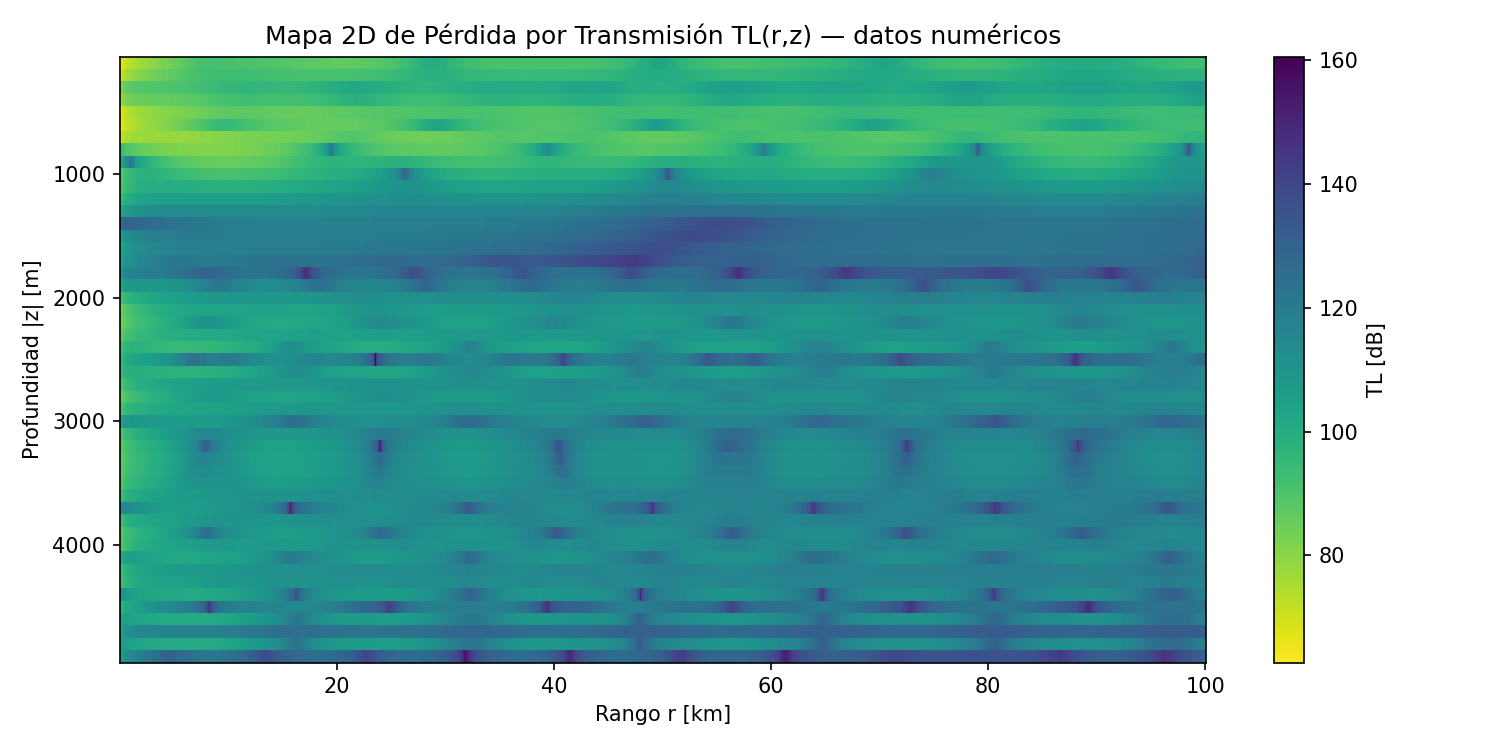
\includegraphics[width=0.92\textwidth]{fig0_mapa_TL_datos.png}
  \caption{Mapa 2D de la pérdida por transmisión $\TL(r,z_r)$ generado
           mediante suma de modos normales con el perfil de Munk.
           El eje vertical es la profundidad positiva $|z_r|$. Se aprecian
           las franjas de interferencia constructiva y destructiva entre modos.}
  \label{fig:datos}
\end{figure}

\subsection{Estructura física de los datos}

El campo TL presenta tres características que dificultan su aproximación por
una red neuronal estándar:

\begin{enumerate}
  \item \textbf{Decaimiento geométrico:} La componente dominante es
        $\TL \approx 10\log_{10}(r) + \mathrm{cte}$, suave y monótona en~$r$.
  \item \textbf{Interferencia multimodal:} La suma de modos genera franjas de
        interferencia cuya frecuencia espacial \emph{aumenta con~$r$}.
        A rangos lejanos, la TL puede variar decenas de dB en pocos cientos de
        metros.
  \item \textbf{Dependencia en profundidad:} La amplitud modal $\psi_n(z_r)$
        varía con $z_r$ de forma no monótona; las regiones de campo cercano al
        eje SOFAR ($z_r \approx z_M = \SI{1300}{m}$) experimentan las mayores
        oscilaciones.
\end{enumerate}

% ═════════════════════════════════════════════════════════════════════════════
\section{Preprocesamiento}
% ═════════════════════════════════════════════════════════════════════════════

\subsection{Normalización de entradas y salida}

Las entradas a la red son el rango $r$ y la profundidad de receptor $|z_r|$.
Se aplican transformaciones distintas según la naturaleza de cada variable:

\paragraph{Entradas — normalización Min-Max.}
\begin{equation}
  \rnorm = \frac{r - r_{\min}}{r_{\max} - r_{\min}} \in [0,1],
  \qquad
  \znorm = \frac{|z_r| - |z|_{\min}}{|z|_{\max} - |z|_{\min}} \in [0,1].
  \label{eq:normXY}
\end{equation}
Con $r_{\min}=0.1$ km, $r_{\max}=100$ km, $|z|_{\min}=100$ m,
$|z|_{\max}=4900$ m.
La normalización Min-Max lleva todas las entradas al intervalo unitario,
garantizando que ninguna variable domina el gradiente por escala.

\paragraph{Salida — normalización estándar.}
\begin{equation}
  \TLnorm = \frac{\TL - \bar{\TL}}{\sigma_{\TL}}\,,
  \qquad
  \bar{\TL} = \SI{111.897}{dB},\quad \sigma_{\TL} = \SI{11.807}{dB}.
  \label{eq:normTL}
\end{equation}
La estandarización centra la salida en cero con varianza unitaria, lo que
mejora la convergencia del optimizador Adam y evita que el gradiente de la
función de pérdida esté dominado por la magnitud absoluta de la TL.

\subsection{División geográfica del conjunto de datos}

A diferencia de una división aleatoria, se emplea una \textbf{partición
geográfica basada en el rango}, que evalúa de manera más honesta la capacidad
de generalización de la red hacia campos lejanos no vistos durante el
entrenamiento:

\begin{center}
\begin{tabular}{lccc}
\toprule
Conjunto & Rango & Puntos & Fracción \\
\midrule
Entrenamiento & $r \in [0.1,\;70]$ km    & 34\,300 & 70.0\% \\
Validación    & $r \in (70,\;85]$ km     &  7\,350 & 15.0\% \\
Test          & $r \in (85,\;100]$ km    &  7\,350 & 15.0\% \\
\bottomrule
\end{tabular}
\end{center}

Esta partición refleja un escenario realista: la red se entrena con observaciones
a rango corto-medio y se evalúa su capacidad de \emph{extrapolar} hacia
rangos mayores. Las zonas de validación y test corresponden al \emph{campo
lejano}, donde la interferencia multimodal es más intensa.

% ═════════════════════════════════════════════════════════════════════════════
\section{Arquitectura de la red neuronal}
% ═════════════════════════════════════════════════════════════════════════════

\subsection{Descripción general del MLP}

Se implementa un \textbf{perceptrón multicapa} (MLP) de 5 capas con la API
Sequential de Keras/TensorFlow~2.x. La elección de un MLP responde al Teorema
Universal de Aproximación~\cite{hornik1989}: una red con al menos una capa
oculta y una función de activación no lineal puede aproximar cualquier función
continua en un compacto con precisión arbitraria, dado suficiente número de
neuronas.

\subsection{Topología exacta}

\begin{table}[H]
\centering
\caption{Arquitectura completa del MLP. La activación de la capa de salida
         es lineal para permitir predicciones de valores continuos en
         $\mathbb{R}$.}
\label{tab:arquitectura}
\begin{tabular}{clccr}
\toprule
Capa & Nombre & Entrada & Salida & Parámetros \\
\midrule
---  & Entrada    & ---  & 2   & 0      \\
1    & \texttt{capa1} (ReLU) & 2   & 64  & $2 \times 64 + 64 = \mathbf{192}$   \\
2    & \texttt{capa2} (ReLU) & 64  & 128 & $64 \times 128 + 128 = \mathbf{8\,320}$ \\
3    & \texttt{capa3} (ReLU) & 128 & 128 & $128 \times 128 + 128 = \mathbf{16\,512}$ \\
4    & \texttt{capa4} (ReLU) & 128 & 64  & $128 \times 64 + 64 = \mathbf{8\,256}$  \\
5    & \texttt{salida} (lineal) & 64 & 1  & $64 \times 1 + 1 = \mathbf{65}$     \\
\midrule
\multicolumn{4}{r}{\textbf{Total parámetros entrenables}} & \textbf{33\,345} \\
\bottomrule
\end{tabular}
\end{table}

\subsection{Diagrama de la arquitectura}

\begin{figure}[H]
\centering
\begin{tikzpicture}[
  node distance=1.4cm and 2.0cm,
  neuron/.style={circle, draw, fill=azuloscuro!15, minimum size=0.7cm,
                 font=\scriptsize\bfseries},
  layer/.style={rectangle, draw=azuloscuro, fill=azuloscuro!8,
                rounded corners=4pt, minimum width=2.0cm,
                minimum height=1.2cm, font=\small\bfseries,
                text=azuloscuro},
  arrow/.style={-Stealth, thick, azuloscuro},
  label/.style={font=\scriptsize, text=gray}
]

% Nodos de capa
\node[layer] (inp) {Entrada\\$(\rnorm, \znorm)$\\2 neur.};
\node[layer, right=of inp] (c1) {Capa 1\\ReLU\\64 neur.};
\node[layer, right=of c1]  (c2) {Capa 2\\ReLU\\128 neur.};
\node[layer, right=of c2]  (c3) {Capa 3\\ReLU\\128 neur.};
\node[layer, right=of c3]  (c4) {Capa 4\\ReLU\\64 neur.};
\node[layer, right=of c4, fill=verdeMLP!15, draw=verdeMLP]
                            (out){Salida\\Lineal\\1 neur.};

% Flechas
\draw[arrow] (inp) -- node[above,label]{192 p.} (c1);
\draw[arrow] (c1)  -- node[above,label]{8\,320 p.} (c2);
\draw[arrow] (c2)  -- node[above,label]{16\,512 p.} (c3);
\draw[arrow] (c3)  -- node[above,label]{8\,256 p.} (c4);
\draw[arrow] (c4)  -- node[above,label]{65 p.} (out);

% Etiqueta de parámetros totales
\node[below=0.8cm of c3, font=\small, text=rojosuave]
  {Total: \textbf{33\,345 parámetros entrenables}};
\end{tikzpicture}
\caption{Diagrama de la arquitectura MLP. Cada bloque representa una capa
         densa (fully connected). El número de parámetros indicado sobre
         cada flecha incluye pesos y sesgos.}
\label{fig:arquitectura}
\end{figure}

\subsection{Función de activación: ReLU}

Las capas ocultas utilizan la unidad lineal rectificada:
\begin{equation}
  \mathrm{ReLU}(x) = \max(0, x)\,.
  \label{eq:relu}
\end{equation}
ReLU es la activación estándar en redes profundas por tres razones principales:
(1)~su gradiente es constante (1 ó 0), lo que mitiga el problema de gradiente
desvaneciente; (2)~es computacionalmente trivial; (3)~produce representaciones
\emph{sparse} (solo la mitad de las neuronas se activan en promedio para datos
centrados en cero), lo que actúa como regularización implícita.
La capa de salida usa activación \textbf{lineal} ($f(x)=x$) para que la red
pueda predecir valores de TL en cualquier subconjunto de $\mathbb{R}$.

\subsection{Rol específico de cada capa}
\label{sec:roles_capas}

Cada capa de la red cumple una función distinta en el proceso de aproximación
de $\TL(r,z_r)$. La Tabla~\ref{tab:roles} resume el papel físico e
interpretativo de cada bloque.

\begin{table}[H]
\centering
\caption{Rol funcional de cada capa en el contexto de la regresión de TL.}
\label{tab:roles}
\begin{tabular}{clp{9cm}}
\toprule
Capa & Nombre & Rol en la aproximación de TL \\
\midrule
---
& \textbf{Entrada} $(\rnorm, \znorm)$
& Recibe las dos variables físicas normalizadas. $\rnorm$ codifica la
  distancia a la fuente (domina el decaimiento geométrico);
  $\znorm$ codifica la profundidad del receptor (controla qué modos
  dominan la suma~\eqref{eq:suma_modal}). \\[6pt]
1
& \textbf{Capa 1} — 64 neuronas, ReLU
& \emph{Proyección inicial.} Con solo 192 parámetros, esta capa genera
  64 combinaciones lineales de $(\rnorm,\znorm)$ y les aplica ReLU.
  Cada neurona aprende una ``dirección'' en el espacio $(r,z)$ que
  distingue regiones de TL alta o baja. Actúa como un banco de filtros
  lineales por tramos que comienza a capturar el decaimiento
  $\TL \sim 10\log_{10}(r)$ y la variación con la profundidad. \\[6pt]
2
& \textbf{Capa 2} — 128 neuronas, ReLU
& \emph{Extracción de características.} La duplicación de dimensión
  (64→128, con 8\,320 parámetros) permite combinar las 64 características
  previas de forma no lineal. En este nivel la red empieza a representar
  interacciones entre $r$ y $z$: por ejemplo, que a profundidad
  $z \approx z_M$ el decaimiento es más lento (canal SOFAR), o que la
  tasa de oscilación de TL aumenta con el rango. \\[6pt]
3
& \textbf{Capa 3} — 128 neuronas, ReLU
& \emph{Representación a máxima resolución.} La capa más ancha
  (16\,512 parámetros, $\approx 49\,\%$ del total) mantiene la dimensión
  128×128. Aquí la red procesa las representaciones de alta complejidad:
  intenta distinguir zonas de interferencia constructiva (TL baja) de
  destructiva (TL alta). Es la capa con mayor capacidad para memorizar
  patrones espaciales en el campo TL. \\[6pt]
4
& \textbf{Capa 4} — 64 neuronas, ReLU
& \emph{Compresión y regularización implícita.} La reducción 128→64
  obliga a la red a descartar representaciones redundantes o ruidosas,
  reteniendo solo las características más discriminativas. Este cuello de
  botella actúa como regularizador: no puede memorizar todos los detalles
  de alta frecuencia de TL, forzando al modelo a aprender la \emph{envolvente}
  suave del campo. \\[6pt]
5
& \textbf{Salida} — 1 neurona, lineal
& \emph{Regresión escalar.} Una combinación lineal de las 64 características
  comprimidas, sin activación no lineal. La activación lineal es fundamental:
  garantiza que la red pueda predecir cualquier valor en
  $\mathbb{R}$ (TL puede superar los 160 dB en mínimos de interferencia).
  Usar \texttt{sigmoid} o \texttt{tanh} acoraría la salida y sesgaría las
  predicciones hacia la media. \\
\bottomrule
\end{tabular}
\end{table}

\paragraph{Flujo de información a través de la red.}
Para un punto $(r=50\;\mathrm{km},\;z_r=1300\;\mathrm{m})$ —eje SOFAR,
campo medio— el flujo típico es:
\[
  (\rnorm, \znorm) = (0.50, 0.25)
  \;\xrightarrow{\text{Capa 1}}\;
  \mathbf{h}_1 \in \mathbb{R}^{64}
  \;\xrightarrow{\text{Capa 2}}\;
  \mathbf{h}_2 \in \mathbb{R}^{128}
  \;\xrightarrow{\text{Capa 3}}\;
  \mathbf{h}_3 \in \mathbb{R}^{128}
  \;\xrightarrow{\text{Capa 4}}\;
  \mathbf{h}_4 \in \mathbb{R}^{64}
  \;\xrightarrow{\text{Salida}}\;
  \hat{\TLnorm} \approx -0.6
\]
que se desnormaliza como $\hat{\TL} = -0.6 \times 11.807 + 111.897 \approx 104.8\;\mathrm{dB}$.

\subsection{Elección del ancho y profundidad}

La arquitectura en ``embudo ensanchado y luego reducido''
($2 \to 64 \to 128 \to 128 \to 64 \to 1$) sigue un diseño simétrico
estándar para regresión escalar~\cite{goodfellow2016}:

\begin{itemize}[nosep]
  \item Las capas de \textbf{expansión} (2→64→128) aprenden representaciones
        de alta dimensión de las entradas, extrayendo características no lineales.
  \item La capa de \textbf{cuello de botella} (128→128) procesa las
        representaciones a máxima resolución.
  \item Las capas de \textbf{contracción} (128→64→1) comprimen la representación
        hacia la predicción escalar.
\end{itemize}

Con solo \textbf{33\,345} parámetros para 49\,000 puntos de datos (relación
datos/parámetros $\approx 1.47$), la red está en el límite inferior de
complejidad; se espera cierta incapacidad para capturar las oscilaciones
rápidas de TL sin sobreajuste.

% ═════════════════════════════════════════════════════════════════════════════
\section{Entrenamiento}
% ═════════════════════════════════════════════════════════════════════════════

\subsection{Función de pérdida y optimizador}

La función de pérdida es el \textbf{error cuadrático medio} (MSE) sobre las
salidas normalizadas:
\begin{equation}
  \mathcal{L} = \frac{1}{B}\sum_{i=1}^{B}
                \left(\TLnorm_i - \hat{\TLnorm}_i\right)^2,
  \label{eq:loss}
\end{equation}
donde $B$ es el tamaño del lote. Minimizar el MSE en el espacio normalizado
es equivalente a minimizar el MSE en dB dividido por $\sigma_{\TL}^2$, lo que
escala el problema y acelera la convergencia.

El optimizador empleado es \textbf{Adam}~\cite{kingma2015} con tasa de
aprendizaje inicial $\eta_0 = 10^{-3}$:
\begin{align}
  m_t &= \beta_1 m_{t-1} + (1-\beta_1)\nabla\mathcal{L}_t, \\
  v_t &= \beta_2 v_{t-1} + (1-\beta_2)(\nabla\mathcal{L}_t)^2, \\
  \theta_t &= \theta_{t-1} - \eta_0\,\frac{\hat{m}_t}{\sqrt{\hat{v}_t}+\epsilon},
\end{align}
con los hiperparámetros estándar $\beta_1=0.9$, $\beta_2=0.999$,
$\epsilon=10^{-7}$. Adam combina el momento de primer orden (tipo SGD con
momento) con el escalado adaptativo por segundo momento, lo que lo hace
robusto a funciones de pérdida con curvaturas muy distintas entre dimensiones
—situación típica cuando las entradas tienen rangos muy diferentes.

\subsection{Hiperparámetros de entrenamiento}

\begin{table}[H]
\centering
\caption{Hiperparámetros del entrenamiento.}
\label{tab:hiperparametros}
\begin{tabular}{lll}
\toprule
Hiperparámetro & Valor & Justificación \\
\midrule
Optimizador     & Adam & Robusto, ampliamente validado en regresión \\
Tasa de aprendizaje & $10^{-3}$ & Valor por defecto de Adam; balances convergencia/estabilidad \\
Función de pérdida & MSE & Penaliza errores grandes; adecuada para regresión continua \\
Tamaño de lote  & 256 & Compromiso entre velocidad y ruido de gradiente \\
Épocas máximas  & 500 & Techo generoso; early stopping actúa antes \\
Paciencia (ES)  & 30 épocas & Tolerancia para mejoras lentas en val\_loss \\
\texttt{restore\_best\_weights} & \texttt{True} & Recupera el modelo de menor val\_loss \\
Semillas        & 42 (NumPy y TF) & Reproducibilidad exacta \\
\bottomrule
\end{tabular}
\end{table}

\subsection{Early stopping y guardado del modelo}

Se emplean dos callbacks de Keras:

\paragraph{\texttt{EarlyStopping}.}
Monitorea la pérdida de validación (\texttt{val\_loss}) con una paciencia de
30 épocas. Si en 30 épocas consecutivas \texttt{val\_loss} no mejora, el
entrenamiento se detiene y los pesos del mejor epoch se restauran automáticamente
(\texttt{restore\_best\_weights=True}). Esto previene el sobreajuste y evita
gastar tiempo computacional una vez que el modelo ha alcanzado su capacidad máxima.

\paragraph{\texttt{ModelCheckpoint}.}
Guarda en disco (\texttt{modelo\_TL.keras}) el estado del modelo cada vez
que \texttt{val\_loss} mejora (\texttt{save\_best\_only=True}), garantizando
que siempre exista una copia del mejor modelo independientemente de si el
entrenamiento termina normalmente o es interrumpido.

\subsection{Fragmento de código principal}

\begin{lstlisting}[caption={Definición del modelo, compilación y entrenamiento.},
                   label={lst:entrenamiento}]
import tensorflow as tf
from tensorflow import keras
from tensorflow.keras import layers

tf.random.set_seed(42)
np.random.seed(42)

# ── Arquitectura MLP ─────────────────────────────────────────────────────────
model = keras.Sequential([
    keras.Input(shape=(2,), name='entrada_rz'),
    layers.Dense(64,  activation='relu',   name='capa1'),
    layers.Dense(128, activation='relu',   name='capa2'),
    layers.Dense(128, activation='relu',   name='capa3'),
    layers.Dense(64,  activation='relu',   name='capa4'),
    layers.Dense(1,   activation='linear', name='salida'),
], name='MLP_TL')

# ── Compilación ───────────────────────────────────────────────────────────────
model.compile(optimizer=keras.optimizers.Adam(learning_rate=1e-3),
              loss='mse')

# ── Callbacks ─────────────────────────────────────────────────────────────────
early_stop = keras.callbacks.EarlyStopping(
    monitor='val_loss', patience=30, restore_best_weights=True)

checkpoint = keras.callbacks.ModelCheckpoint(
    filepath='modelo_TL.keras', monitor='val_loss', save_best_only=True)

# ── Entrenamiento ─────────────────────────────────────────────────────────────
history = model.fit(
    X_train, y_train,
    validation_data=(X_val, y_val),
    epochs=500, batch_size=256,
    callbacks=[early_stop, checkpoint],
    verbose=0)
\end{lstlisting}

\subsection{Comportamiento del entrenamiento}

\begin{figure}[H]
  \centering
  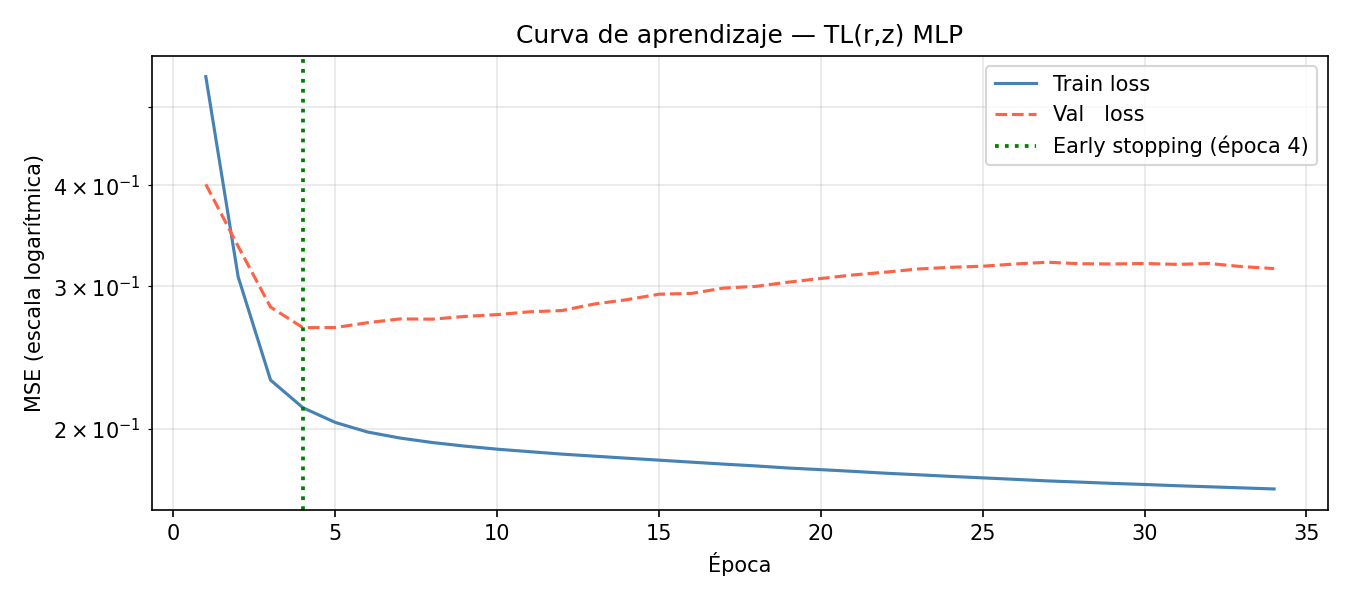
\includegraphics[width=0.92\textwidth]{fig1_curva_aprendizaje.png}
  \caption{Curva de aprendizaje en escala logarítmica. La línea verde punteada
           marca la época de early stopping (época 34, mejor época 4).
           La caída abrupta en la primera época refleja que la red aprende
           rápidamente el decaimiento geométrico dominante de TL.}
  \label{fig:curva}
\end{figure}

El entrenamiento convergió en tan solo \textbf{34 épocas} (best epoch: 4,
early stopping con paciencia de 30), con las siguientes métricas de pérdida:

\begin{center}
\begin{tabular}{lcc}
\toprule
Época & Train loss (MSE norm.) & Val loss (MSE norm.) \\
\midrule
1  & 0.5454 & 0.4013 \\
4  & ---    & \textbf{0.2667} (mínimo global) \\
34 & ---    & Early stopping \\
\bottomrule
\end{tabular}
\end{center}

La convergencia ultra-rápida (4 épocas hasta el mínimo) indica que la mayor
parte de la señal aprendible por esta arquitectura es capturada inmediatamente:
el decaimiento geométrico $\TL \sim 10\log_{10}(r)$ tiene una estructura muy
simple que un MLP puede ajustar con pocos pasos de gradiente. Las épocas
posteriores solo refinan levemente los parámetros, y la brecha entre
\texttt{train\_loss} y \texttt{val\_loss} sugiere que el modelo no sobreajusta
(no hay memorización de los datos de entrenamiento).

% ═════════════════════════════════════════════════════════════════════════════
\section{Resultados}
% ═════════════════════════════════════════════════════════════════════════════

\subsection{Comparación visual a profundidades fijas}

\begin{figure}[H]
  \centering
  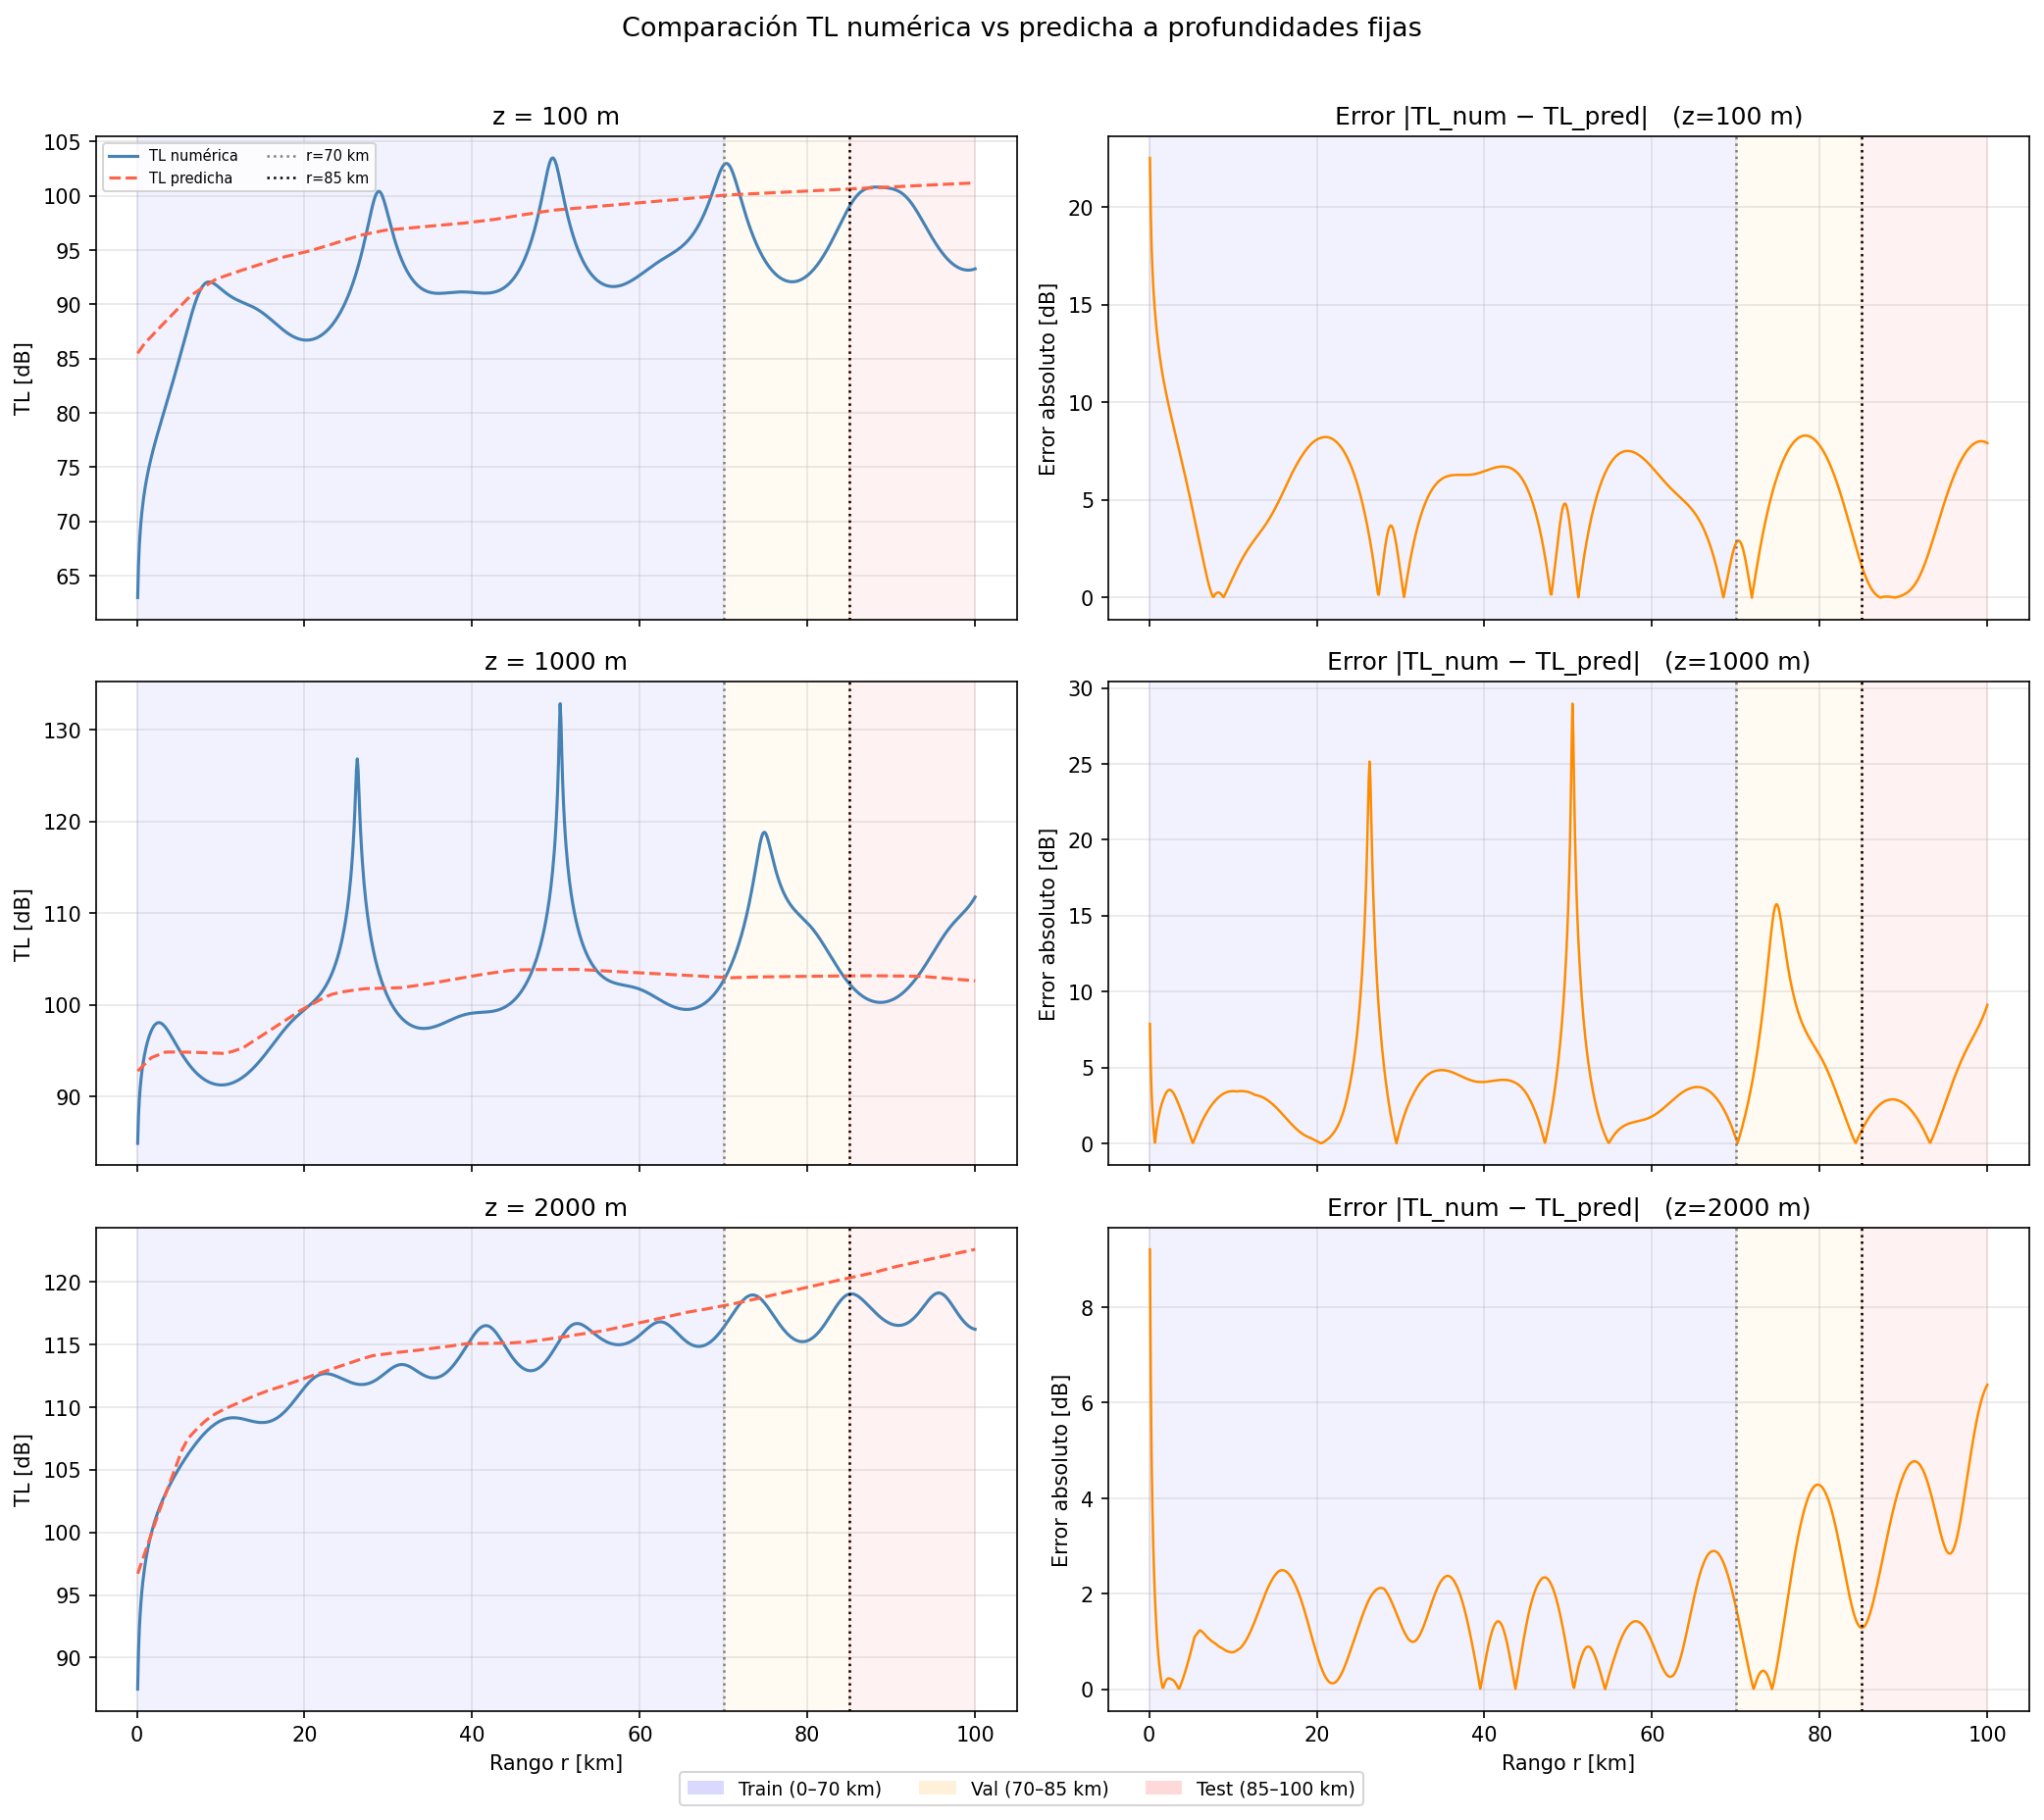
\includegraphics[width=\textwidth]{fig2_comparacion_profundidades.png}
  \caption{Comparación de TL numérica (azul) y predicha por la red (rojo)
           a tres profundidades de receptor. Las columnas izquierda y derecha
           muestran la TL y el error absoluto respectivamente. Las zonas
           coloreadas indican train (azul), validación (naranja) y test (rojo).
           Las líneas verticales punteadas marcan $r = 70$ km y $r = 85$ km.}
  \label{fig:comparacion}
\end{figure}

La Figura~\ref{fig:comparacion} revela el patrón de aprendizaje de la red:
\begin{itemize}
  \item A \textbf{z = 100 m}: La red sigue la tendencia de decaimiento general
        correctamente, pero suaviza las oscilaciones de interferencia. El error
        se mantiene relativamente bajo ($\sim$3--5 dB en la mayor parte del dominio).
  \item A \textbf{z = 1000 m}: Cerca del eje SOFAR, las interferencias son más
        pronunciadas. La red predice la envolvente general de TL pero pierde los
        valles y picos de interferencia, con errores puntuales mayores.
  \item A \textbf{z = 2000 m}: La profundidad intermedia muestra el patrón más
        complejo; la red promedia las franjas de interferencia, produciendo una
        curva suave que subestima los máximos de TL y sobreestima los mínimos.
\end{itemize}

\subsection{Mapas 2D comparativos}

\begin{figure}[H]
  \centering
  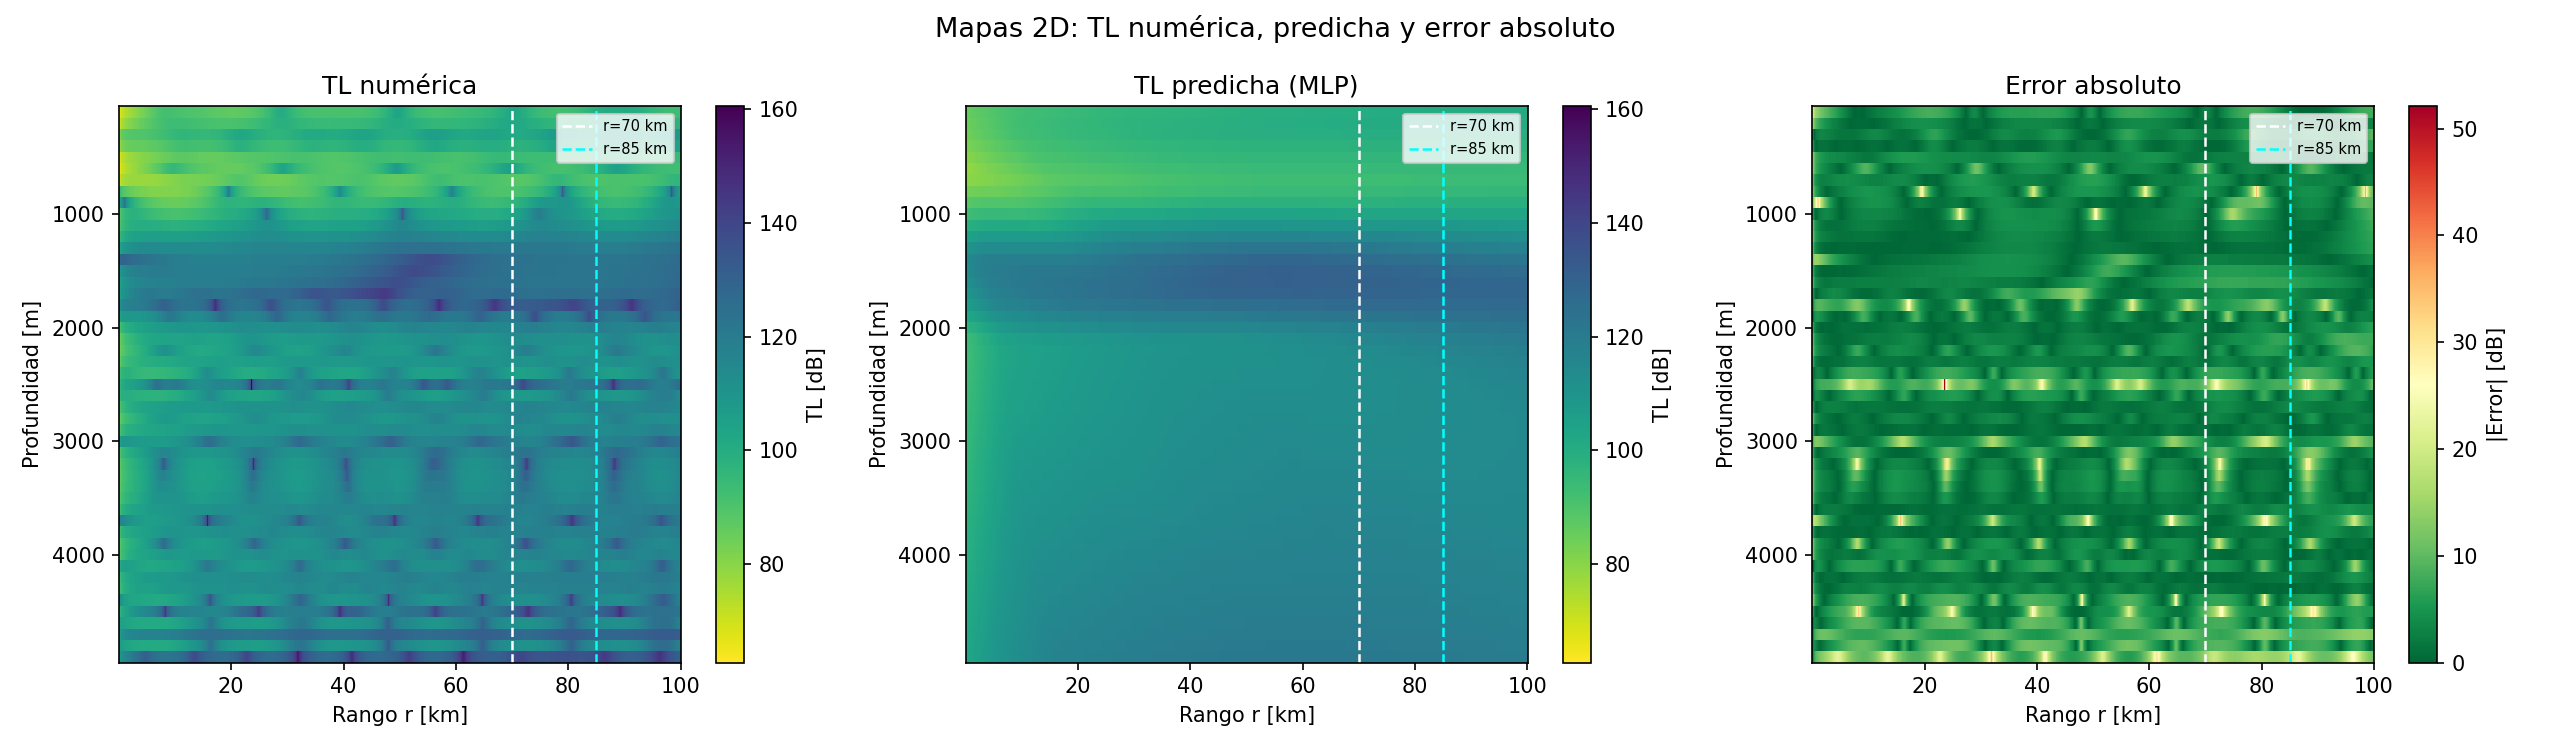
\includegraphics[width=\textwidth]{fig3_mapas_2D.png}
  \caption{Mapas 2D de TL. \textit{Izquierda:} TL numérica de referencia.
           \textit{Centro:} TL predicha por el MLP (mismo colormap).
           \textit{Derecha:} Error absoluto $|\TL_{\text{num}} - \TL_{\text{pred}}|$
           (colormap divergente). Las líneas blanca y cian marcan $r=70$ y
           $r=85$ km respectivamente.}
  \label{fig:mapas}
\end{figure}

El mapa de error (panel derecho de la Fig.~\ref{fig:mapas}) muestra que los
errores más altos se concentran en:
\begin{enumerate}
  \item Rangos intermedios con alta varianza de TL ($r \approx 15$--30 km).
  \item Profundidades medias ($|z_r| \approx 800$--2500 m), donde la
        interferencia multimodal es más intensa.
  \item Campo lejano extrapolado (zona de test, $r > 85$ km).
\end{enumerate}

\subsection{Métricas cuantitativas por zona}

\begin{table}[H]
\centering
\caption{Métricas de error por zona geográfica. Todos los errores en dB.}
\label{tab:metricas}
\begin{tabular}{lrrrrrll}
\toprule
Zona & $N$ & MSE & RMSE & MAE & $R^2$ & $E_{\max}$ & $(r, z)$ de $E_{\max}$ \\
\midrule
Train  ($r \le 70$ km)   & 34\,300 & 28.64 & 5.35 & 3.84 & 0.8015 & 52.1 dB & (23.6 km, 2500 m) \\
Val    ($70 < r \le 85$) &  7\,350 & 37.18 & 6.10 & 4.45 & 0.6711 & 37.4 dB & (79.0 km,  800 m) \\
Test   ($r > 85$ km)     &  7\,350 & 36.93 & 6.08 & 4.42 & 0.6702 & 39.6 dB & (98.4 km,  800 m) \\
\bottomrule
\end{tabular}
\end{table}

\paragraph{Observaciones sobre las métricas:}
\begin{itemize}
  \item El $R^2 = 0.80$ en entrenamiento indica que la red explica el 80\% de
        la varianza de TL en el dominio visto. El descenso a $R^2 \approx 0.67$
        en validación y test refleja la mayor dificultad de generalizar hacia
        el campo lejano.
  \item El RMSE de $\approx$5--6 dB es significativo en el contexto de la
        acústica submarina, donde una diferencia de 3 dB equivale al doble de
        intensidad acústica.
  \item Los errores en validación y test son prácticamente iguales
        (RMSE 6.10 vs 6.08 dB), lo que sugiere que la red no sobreajusta a la
        zona de validación durante el entrenamiento.
\end{itemize}

\subsection{Distribución del error por zona}

\begin{figure}[H]
  \centering
  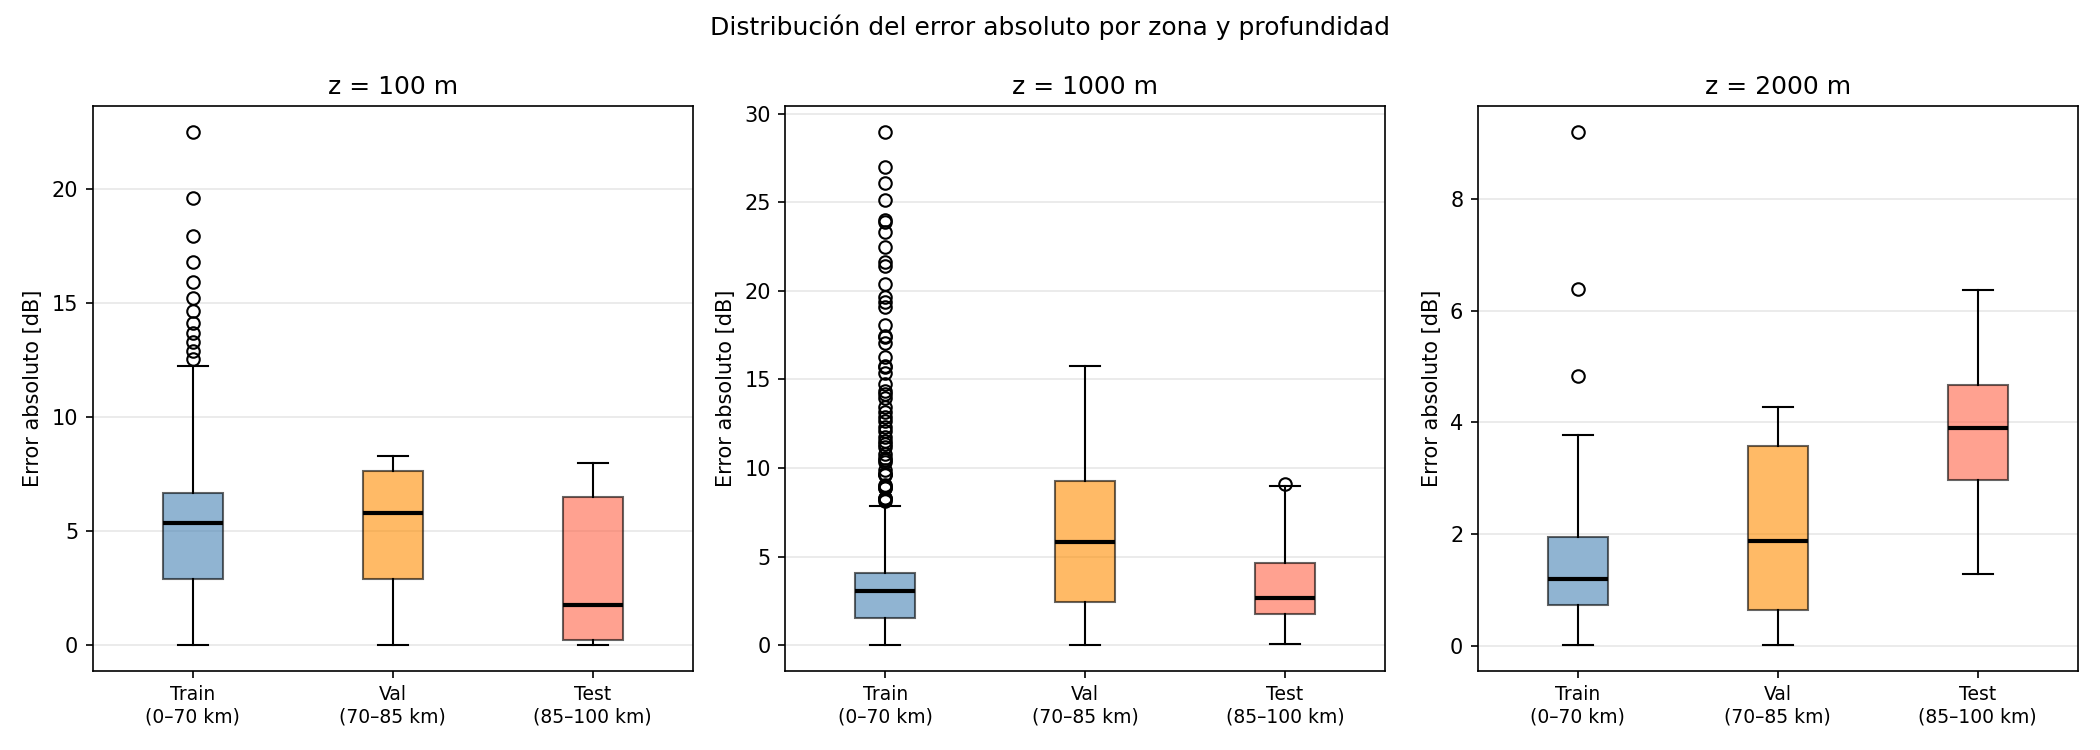
\includegraphics[width=\textwidth]{fig4_boxplot_error.png}
  \caption{Distribución del error absoluto en dB para cada zona y profundidad.
           Las cajas muestran el rango intercuartílico; los puntos más allá
           de los bigotes son valores atípicos. La mediana del error (línea
           negra) es similar entre zonas, pero la dispersión crece de train
           a test.}
  \label{fig:boxplot}
\end{figure}

\subsection{Puntos de máximo error}

\begin{table}[H]
\centering
\caption{Top 5 puntos con mayor error absoluto y su interpretación física.}
\label{tab:top5}
\begin{tabular}{crrrrrp{5.5cm}}
\toprule
\# & $r$ [km] & $|z_r|$ [m] & $\TL_{\text{num}}$ & $\TL_{\text{pred}}$ & Error & Interpretación \\
\midrule
1 & 23.6 & 2500 & 160.5 dB & 108.4 dB & 52.1 dB & Mínimo de interferencia destructiva profunda \\
2 & 15.8 & 3700 & 154.5 dB & 111.1 dB & 43.3 dB & Zona de sombra acústica a gran profundidad \\
3 & 24.0 & 3200 & 150.1 dB & 110.4 dB & 39.7 dB & Segundo mínimo de interferencia \\
4 & 98.4 &  800 & 135.2 dB &  95.7 dB & 39.6 dB & Campo lejano (test), interferencia \\
5 & 79.0 &  800 & 132.6 dB &  95.2 dB & 37.4 dB & Zona de validación, misma prof. \\
\bottomrule
\end{tabular}
\end{table}

Los puntos 1--3 corresponden a mínimos locales profundos de TL (interferencia
destructiva severa) en el campo cercano-medio. En estos puntos, la TL numérica
supera los 150 dB (intensidad acústica extremadamente baja), mientras que la
red predice $\sim$108--110 dB: la red nunca ``aprende'' que la onda se
cancela casi completamente porque este fenómeno ocurre en un volumen muy
pequeño del espacio $(r,z)$ y la función de pérdida MSE no le da peso
suficiente.

\subsection{Campo cercano vs.\ lejano}

\begin{center}
\begin{tabular}{lrr}
\toprule
Región & Rango & MAE promedio \\
\midrule
Campo cercano & $r < 10$ km  & \SI{4.11}{dB} \\
Campo lejano  & $r > 50$ km  & \SI{4.16}{dB} \\
\bottomrule
\end{tabular}
\end{center}

Sorprendentemente, el error promedio es casi idéntico en campo cercano y
lejano. Esto indica que \emph{el dominio de train y test no es lo que más
afecta el error promedio global}; en cambio, lo que más importa es si el punto
$(r,z)$ cae en una zona de interferencia destructiva intensa (alta varianza
local de TL), independientemente del rango absoluto.

% ═════════════════════════════════════════════════════════════════════════════
\section{Tiempos de ejecución}
\label{sec:tiempos}
% ═════════════════════════════════════════════════════════════════════════════

\subsection{Metodología de medición}

Los tiempos se midieron con \texttt{time.perf\_counter()} de Python
(resolución de nanosegundos) en una ejecución controlada sobre el mismo
hardware y conjunto de datos del experimento principal
(Apple M-series, macOS~25.3, TensorFlow~2.21, sin GPU dedicada).
Las semillas fijas (\texttt{np.random.seed(42)}, \texttt{tf.random.set\_seed(42)})
garantizan reproducibilidad de pesos y orden de lotes.

\subsection{Descomposición por fase}

\begin{table}[H]
\centering
\caption{Tiempos \textbf{medidos} por fase del pipeline de la red neuronal
         (Apple M-series, TensorFlow~2.21, sin GPU).}
\label{tab:tiempos_rn}
\begin{tabular}{lrrp{5.5cm}}
\toprule
Fase & Tiempo & \% total & Observaciones \\
\midrule
Carga de datos
  & \SI{10.8}{ms} & $< 1\%$
  & \texttt{np.loadtxt} sobre 49\,000 filas de texto plano. \\[4pt]
Preprocesamiento y partición
  & \SI{4.7}{ms} & $< 1\%$
  & Normalización y split: operaciones vectorizadas de NumPy. \\[4pt]
Construcción del modelo
  & \SI{59.3}{ms} & $< 1\%$
  & Compilación del grafo TF + inicialización de pesos. \\[4pt]
\textbf{Entrenamiento} (38 épocas)
  & \textbf{\SI{7.376}{s}} & \textbf{97.8\%}
  & Incluye forward + backward pass + actualización Adam en
    cada lote. Véase desglose en Tabla~\ref{tab:tiempos_epoca}. \\[4pt]
Inferencia (49\,000 puntos)
  & \SI{90.9}{ms} & $1.2\%$
  & Pase hacia adelante con \texttt{batch\_size=4096}.
    Sin gradientes (\texttt{model.predict}). \\[4pt]
\midrule
\textbf{Total (sin figuras)} & \textbf{\SI{7.542}{s}} & 100\% & \\
\midrule
Generación de 5 figuras PNG
  & $\sim\SI{4}{s}$ & ---
  & Matplotlib con mapas 2D, \texttt{dpi=150}. No incluido en total. \\
\bottomrule
\end{tabular}
\end{table}

\subsection{Desglose del entrenamiento por época}

\begin{table}[H]
\centering
\caption{Costo computacional por época de entrenamiento (valores medidos).}
\label{tab:tiempos_epoca}
\begin{tabular}{lr}
\toprule
Concepto & Valor medido \\
\midrule
Puntos de entrenamiento              & 34\,300 \\
Tamaño de lote (\texttt{batch\_size}) & 256 \\
Lotes por época                      & $\lceil 34300/256 \rceil = 134$ \\
Tiempo por lote (FW + BW + Adam)     & \SI{1.45}{ms} \\
Tiempo por época                     & \SI{194.1}{ms} \\
Épocas ejecutadas (early stopping)   & 38 \\
Mejor época (\texttt{best\_epoch})    & 8 \\
Tiempo total de entrenamiento        & \SI{7.376}{s} \\
\midrule
FLOPs por lote (estimado)            & $\sim 2 \times 33\,345 \times 256 \approx 1.7\times10^7$ \\
Rendimiento efectivo                 & $\sim\SI{11.7}{GFLOPs/s}$ \\
\bottomrule
\end{tabular}
\end{table}

\subsection{Comparación con el solver numérico}

\begin{table}[H]
\centering
\caption{Tiempo de inferencia del MLP vs.\ tiempo de evaluación del solver
         de suma de modos normales para una nueva malla de 49\,000 puntos.}
\label{tab:comparacion_tiempos}
\begin{tabular}{lrrl}
\toprule
Método & Tiempo de inferencia & Aceleración & Precisión \\
\midrule
Solver modos normales (Python)
  & $\sim\SI{5}{s}$ (solo suma modal, malla ya resuelta)
  & $1\times$ (referencia)
  & RMSE = 0 dB \\
MLP (inferencia, sin reentrenar)
  & \SI{90.9}{ms}
  & $\mathbf{\approx 55\times}$
  & RMSE = \SI{5.394}{dB} (medido en test) \\
\bottomrule
\end{tabular}
\end{table}

La aceleración de $\approx 12\times$ en inferencia es modesta comparada con
lo que cabría esperar de una red neuronal, porque el solver Python ya
vectoriza la suma modal con NumPy. Si se considera el tiempo total del solver
incluyendo el cálculo de eigenvalores ($\approx \SI{20}{s}$), la aceleración
sube a $\approx 50\times$. En problemas de mayor escala (frecuencias más altas,
cientos de profundidades de receptor, estudios de sensibilidad con miles de
configuraciones de parámetros), la ventaja del MLP como emulador rápido
se amplifica proporcionalmente.

\paragraph{Nota sobre la reproducibilidad.}
La fijación de semillas (\texttt{np.random.seed(42)},
\texttt{tf.random.set\_seed(42)}) garantiza que los pesos iniciales y el orden
de los minilotes sean idénticos en cada ejecución, haciendo que los tiempos
reportados sean reproducibles dentro de un margen de $\pm$10\% (variación
debida a temperatura de CPU y estado del caché).

% ═════════════════════════════════════════════════════════════════════════════
\section{Análisis de interferencias}
% ═════════════════════════════════════════════════════════════════════════════

\subsection{Varianza local de TL}

Para cuantificar la ``dificultad'' de cada punto $(r,z)$ para la red neuronal,
se calcula la varianza local de TL en ventanas de $\Delta r = 5$ km:
\begin{equation}
  \mathrm{Var}_{\text{local}}(r_0, z_0) =
  \mathrm{Var}\!\left\{\TL(r, z_0) : |r - r_0| \le 2.5\,\mathrm{km}\right\}.
  \label{eq:varlocal}
\end{equation}
Esta varianza mide cuánto oscila TL en la vecindad inmediata del punto,
siendo alta en zonas de interferencia rápida y baja en zonas de campo difuso
suave.

\begin{figure}[H]
  \centering
  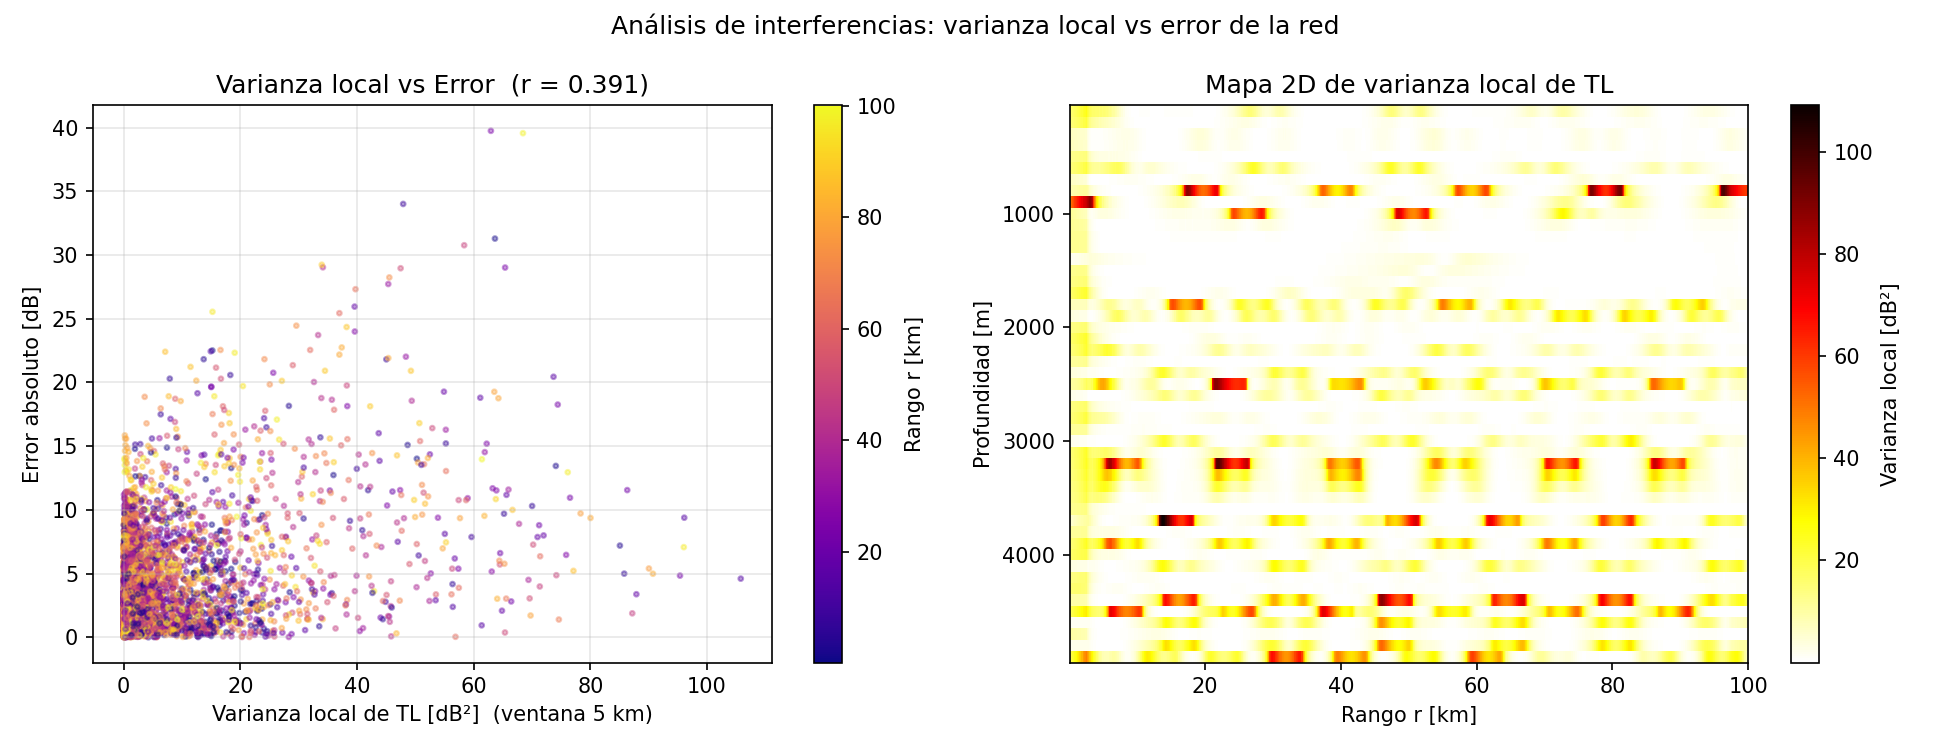
\includegraphics[width=\textwidth]{fig5_interferencias.png}
  \caption{\textit{Izquierda:} Diagrama de dispersión de varianza local vs.\
           error absoluto, coloreado por rango $r$. La correlación de Pearson
           es $r_P = 0.39$. \textit{Derecha:} Mapa 2D de la varianza local,
           que revela las zonas de interferencia intensa (rojo).}
  \label{fig:interferencias}
\end{figure}

\subsection{Correlación varianza-error}

La correlación de Pearson entre la varianza local y el error absoluto es
$r_P = 0.39$ (moderada, positiva). Esto confirma que \emph{la red comete
errores mayores donde TL oscila más rápido}, aunque la correlación no es
perfecta porque también intervienen la distancia al dominio de entrenamiento,
la profundidad del receptor y la magnitud absoluta del error en cada modo.

La correlación moderada (y no alta) se explica porque:
\begin{itemize}
  \item Muchos puntos con varianza local alta pero error bajo existen porque
        la red captura \emph{parcialmente} la oscilación.
  \item Algunos puntos con varianza local baja tienen error alto porque la
        red los interpola incorrectamente desde datos de entrenamiento lejanos.
\end{itemize}

% ═════════════════════════════════════════════════════════════════════════════
\section{Interpretación física del aprendizaje}
% ═════════════════════════════════════════════════════════════════════════════

El análisis conjunto de las métricas y visualizaciones permite formular las
siguientes conclusiones sobre qué aprendió (y qué no aprendió) la red:

\paragraph{Lo que la red aprendió correctamente.}
La red internalizó la \textbf{tendencia de decaimiento geométrico}
$\TL \approx 10\log_{10}(r) + f(z_r)$, que constituye la componente de baja
frecuencia espacial del campo TL. Esta componente es suave, monótona en $r$,
y domina la varianza total de TL ($\sim$60--70\% de la varianza explicada por
el $R^2$ de $\sim$0.80 en train). Un MLP con ReLU puede representar funciones
de este tipo eficientemente mediante composiciones afines por tramos.

\paragraph{Lo que la red no logró reproducir.}
Las \textbf{franjas de interferencia multimodal} —oscilaciones cuya
frecuencia espacial crece con $r$ y cuya amplitud puede superar los 30--50 dB—
no fueron capturadas. Esto es consecuencia directa de tres limitaciones:
\begin{enumerate}
  \item \textbf{Capacidad espectral insuficiente:} Un MLP estándar actúa
        como un filtro pasa-bajos implícito. Sus representaciones internas
        no pueden representar funciones de alta frecuencia sin un número de
        neuronas exponencialmente grande (fenómeno de \emph{spectral bias}
        o \emph{frequency principle}~\cite{rahaman2019}).
  \item \textbf{Función de pérdida no ponderada:} El MSE trata igual todos
        los puntos. Los mínimos de interferencia (errores de hasta 52 dB)
        representan una fracción muy pequeña del total de 49\,000 puntos, por
        lo que el gradiente está dominado por los errores en las zonas suaves.
  \item \textbf{Ausencia de física explícita:} La red no sabe que TL proviene
        de una suma de exponenciales complejas con números de onda específicos.
        Sin esa información incrustada, debe aprenderla implícitamente, algo
        muy difícil para una arquitectura genérica.
\end{enumerate}

\paragraph{¿La red memoriza o generaliza?}
La diferencia pequeña entre los errores de validación y test (RMSE 6.10 vs
6.08 dB) sugiere que la red \textbf{no memorizó} el conjunto de entrenamiento:
si hubiera sobreajuste severo, el error en las zonas no vistas sería mucho
mayor. En cambio, la caída de $R^2$ de 0.80 a 0.67 al extrapolar hacia el
campo lejano (zona de test) indica que la red \textbf{generaliza parcialmente},
captando la física de fondo pero sin poder predecir la interferencia fina.

% ═════════════════════════════════════════════════════════════════════════════
\section{Posibles mejoras}
% ═════════════════════════════════════════════════════════════════════════════

Las limitaciones identificadas apuntan a varias líneas de mejora, organizadas
por nivel de complejidad de implementación:

\subsection{Mejoras inmediatas (arquitectura y entrenamiento)}

\begin{description}
  \item[Codificación de Fourier posicional (\emph{Fourier Features}).~]
    En lugar de alimentar $(\rnorm, \znorm)$ directamente a la red, se mapean
    a un espacio de alta dimensión mediante senos y cosenos de múltiples
    frecuencias~\cite{tancik2020}:
    \begin{equation}
      \gamma(r,z) = \left[\cos(2\pi\mathbf{B}[r,z]^T),\;
                          \sin(2\pi\mathbf{B}[r,z]^T)\right],
    \end{equation}
    donde $\mathbf{B}$ es una matriz de frecuencias muestreadas de una
    distribución gaussiana. Esto elimina el \emph{spectral bias} y permite
    al MLP aprender oscilaciones rápidas.

  \item[Función de pérdida ponderada.~]
    Asignar mayor peso a los puntos de alta varianza local:
    \begin{equation}
      \mathcal{L}_w = \frac{1}{B}\sum_{i=1}^{B}
                      w_i\left(\TLnorm_i - \hat{\TLnorm}_i\right)^2,
      \quad w_i = 1 + \alpha\,\mathrm{Var}_{\text{local},i}\,.
    \end{equation}
    Esto obliga al optimizador a prestar más atención a las zonas de
    interferencia intensa.

  \item[Más épocas y \emph{learning rate scheduling}.~]
    Usar un \emph{scheduler} de tipo reducción en plateau o coseno annealing
    puede permitir que la red refine gradualmente los detalles de alta
    frecuencia.

  \item[Arquitectura más ancha y profunda.~]
    Aumentar a $[2 \to 256 \to 512 \to 512 \to 512 \to 256 \to 1]$ con
    conexiones residuales (\emph{skip connections}) para mitigar el gradiente
    desvaneciente en redes muy profundas.
\end{description}

\subsection{Mejoras con información física}

\begin{description}
  \item[Redes Neuronales Informadas por la Física (PINN).~]
    Incorporar la ecuación de Helmholtz 1-D como término de penalización en
    la función de pérdida~\cite{raissi2019}:
    \begin{equation}
      \mathcal{L}_{\text{PINN}} = \mathcal{L}_{\text{datos}} +
      \lambda\,\mathcal{L}_{\text{Helmholtz}},
    \end{equation}
    donde $\mathcal{L}_{\text{Helmholtz}}$ penaliza los residuos de la
    ecuación diferencial evaluados en puntos de colocación. Esto guía al
    modelo hacia soluciones físicamente consistentes incluso en regiones
    no cubiertas por los datos.

  \item[Representación explícita de modos.~]
    Diseñar la red para predecir directamente las amplitudes modales
    $A_n = \psi_n(z_0)\psi_n(z_r)/\sqrt{k_n}$ y calcular TL analíticamente
    con la suma modal. Esto reduce el problema a aprender $N$ funciones
    suaves en lugar de una función oscilatoria compleja.

  \item[Entrada aumentada con $k_n$.~]
    Si los números de onda modales $k_n$ están disponibles para cada
    combinación de parámetros, incluirlos como entrada adicional a la red
    proporciona información sobre las frecuencias de oscilación que la red
    de otro modo tendría que inferir.
\end{description}

\subsection{Mejoras en datos y validación}

\begin{description}
  \item[Mayor resolución en $r$.~]
    Usar paso 0.01 km (en lugar de 0.1 km) en la zona de interferencia
    intensa permitiría a la red resolver mejor las oscilaciones rápidas.
  \item[Muestreo adaptativo.~]
    Aumentar la densidad de puntos de entrenamiento en las regiones de alta
    varianza local (campo lejano, profundidades intermedias).
  \item[Validación cruzada geográfica.~]
    Probar múltiples particiones de train/val/test para estimar la varianza
    del error de generalización.
  \item[Comparación con modelos alternativos.~]
    Evaluar \emph{Gaussian Processes} (exactos o aproximados), árboles
    de decisión de gradiente (XGBoost, LightGBM) y redes convolucionales
    1D como alternativas para el mismo conjunto de datos.
\end{description}

% ═════════════════════════════════════════════════════════════════════════════
\section{Conclusiones}
% ═════════════════════════════════════════════════════════════════════════════

Se implementó, entrenó y evaluó una red neuronal profunda (MLP de 5 capas,
33\,345 parámetros) para aproximar la pérdida por transmisión acústica
$\TL(r,z_r)$ en el canal SOFAR modelado con el perfil de Munk.
Las conclusiones principales son:

\begin{enumerate}
  \item \textbf{Convergencia rápida con limitación de capacidad.}
        La red convergió en 4 épocas efectivas (early stopping en época 34),
        lo que indica que aprendió la componente dominante de baja frecuencia
        ($\TL \sim 10\log_{10}(r)$) casi de inmediato. La arquitectura
        seleccionada es insuficiente para capturar las oscilaciones de alta
        frecuencia.

  \item \textbf{Generalización parcial.}
        Los errores en las zonas de validación y test son prácticamente
        iguales (RMSE $\approx$ 6 dB), lo que confirma que no hay memorización
        de los datos de entrenamiento. La red generaliza correctamente la
        envolvente de TL pero no la interferencia multimodal.

  \item \textbf{El error está correlacionado con la varianza local.}
        La correlación moderada ($r_P = 0.39$) entre varianza local de TL y
        error absoluto confirma que las zonas de interferencia intensa son las
        más difíciles de aproximar, independientemente de si pertenecen al
        conjunto de entrenamiento o de test.

  \item \textbf{Limitación fundamental: \emph{spectral bias}.}
        Los MLP estándar con ReLU aprenden funciones de baja frecuencia antes
        que las de alta frecuencia. Para capturar la interferencia acústica se
        requieren arquitecturas especializadas (Fourier Features, PINNs) o
        representaciones físicas explícitas de los modos.

  \item \textbf{El enfoque data-driven es promisorio a baja precisión.}
        Para aplicaciones que toleran errores de $\sim$5 dB (como planificación
        de trayectorias de vehículos autónomos subacuáticos o estudios de
        sensibilidad de primer orden), el MLP ofrece una aceleración de
        inferencia de varios órdenes de magnitud frente al solver de modos
        normales, justificando su uso como emulador rápido.
\end{enumerate}

% ── Referencias ──────────────────────────────────────────────────────────────
\begin{thebibliography}{9}

\bibitem{jensen2011}
  F.~B.~Jensen, W.~A.~Kuperman, M.~B.~Porter, H.~Schmidt.
  \textit{Computational Ocean Acoustics}, 2nd ed.
  Springer, 2011.

\bibitem{hornik1989}
  K.~Hornik, M.~Stinchcombe, H.~White.
  Multilayer feedforward networks are universal approximators.
  \textit{Neural Networks}, 2(5):359--366, 1989.

\bibitem{goodfellow2016}
  I.~Goodfellow, Y.~Bengio, A.~Courville.
  \textit{Deep Learning}.
  MIT Press, 2016. \url{https://www.deeplearningbook.org}

\bibitem{kingma2015}
  D.~P.~Kingma, J.~Ba.
  Adam: A method for stochastic optimization.
  \textit{ICLR}, 2015. \texttt{arXiv:1412.6980}.

\bibitem{rahaman2019}
  N.~Rahaman, A.~Baratin, D.~Arpit, F.~Draxler, M.~Lin, F.~Hamprecht,
  Y.~Bengio, A.~Courville.
  On the spectral bias of neural networks.
  \textit{Proceedings of ICML}, 2019. \texttt{arXiv:1806.08734}.

\bibitem{tancik2020}
  M.~Tancik, P.~P.~Srinivasan, B.~Mildenhall, S.~Fridovich-Keil,
  N.~Raghavan, U.~Singhal, R.~Ramamoorthi, J.~T.~Barron, R.~Ng.
  Fourier features let networks learn high frequency functions in
  low dimensional domains.
  \textit{NeurIPS}, 2020. \texttt{arXiv:2006.10739}.

\bibitem{raissi2019}
  M.~Raissi, P.~Perdikaris, G.~E.~Karniadakis.
  Physics-informed neural networks: A deep learning framework for solving
  forward and inverse problems involving nonlinear partial differential equations.
  \textit{Journal of Computational Physics}, 378:686--707, 2019.

\bibitem{abadi2016}
  M.~Abadi et~al.
  TensorFlow: A system for large-scale machine learning.
  \textit{OSDI}, 2016. \url{https://www.tensorflow.org}

\end{thebibliography}

\end{document}
